\providecommand{\main}{..}
\documentclass[\main/thesis.tex]{subfiles}

\begin{document}
\begin{appendices}
\chapter{Label-wise Feature Importances for XGBoost Classifiers with Autoencoder Embeddings}

In an extension of Section~\ref{sec:xgb_aenc_results}, I provide a categorical breakdown of the feature utilization from Configuration~\ref{item:xgb_aenc_model_top_1000_w_embd} in Figure~\ref{fig:xgb_aenc_top_1000_features_labelwise}, as well as Configuration~\ref{item:xgb_aenc_model_top_100_w_embd} displayed in Figure~\ref{fig:xgb_aenc_top_100_features_labelwise}.

Feature utilization is a value ranging between $[0, 1]$ that represents how many features from the given category is used in the pruned classifier.
For example, consider the meta variable \emph{Age}.
Within an \gls{ecg} record, there is only 1 tabular feature representing patient age.
A utilization of $1$ means that age is always determined to be an important feature to be kept.
Consider another category \emph{Heart Rate}.
Referring to Section~\ref{ssec:xgb_feature_engineering}, we know that any given lead may contribute at most 53 heart rate variability features.
A utilization of $0.4$ means that only 21 of the available 53 features generated from the lead were deemed important and kept in the pruned classifier input space.

\begin{figure}[t]
    \centering
    \makebox[\textwidth][c]{
        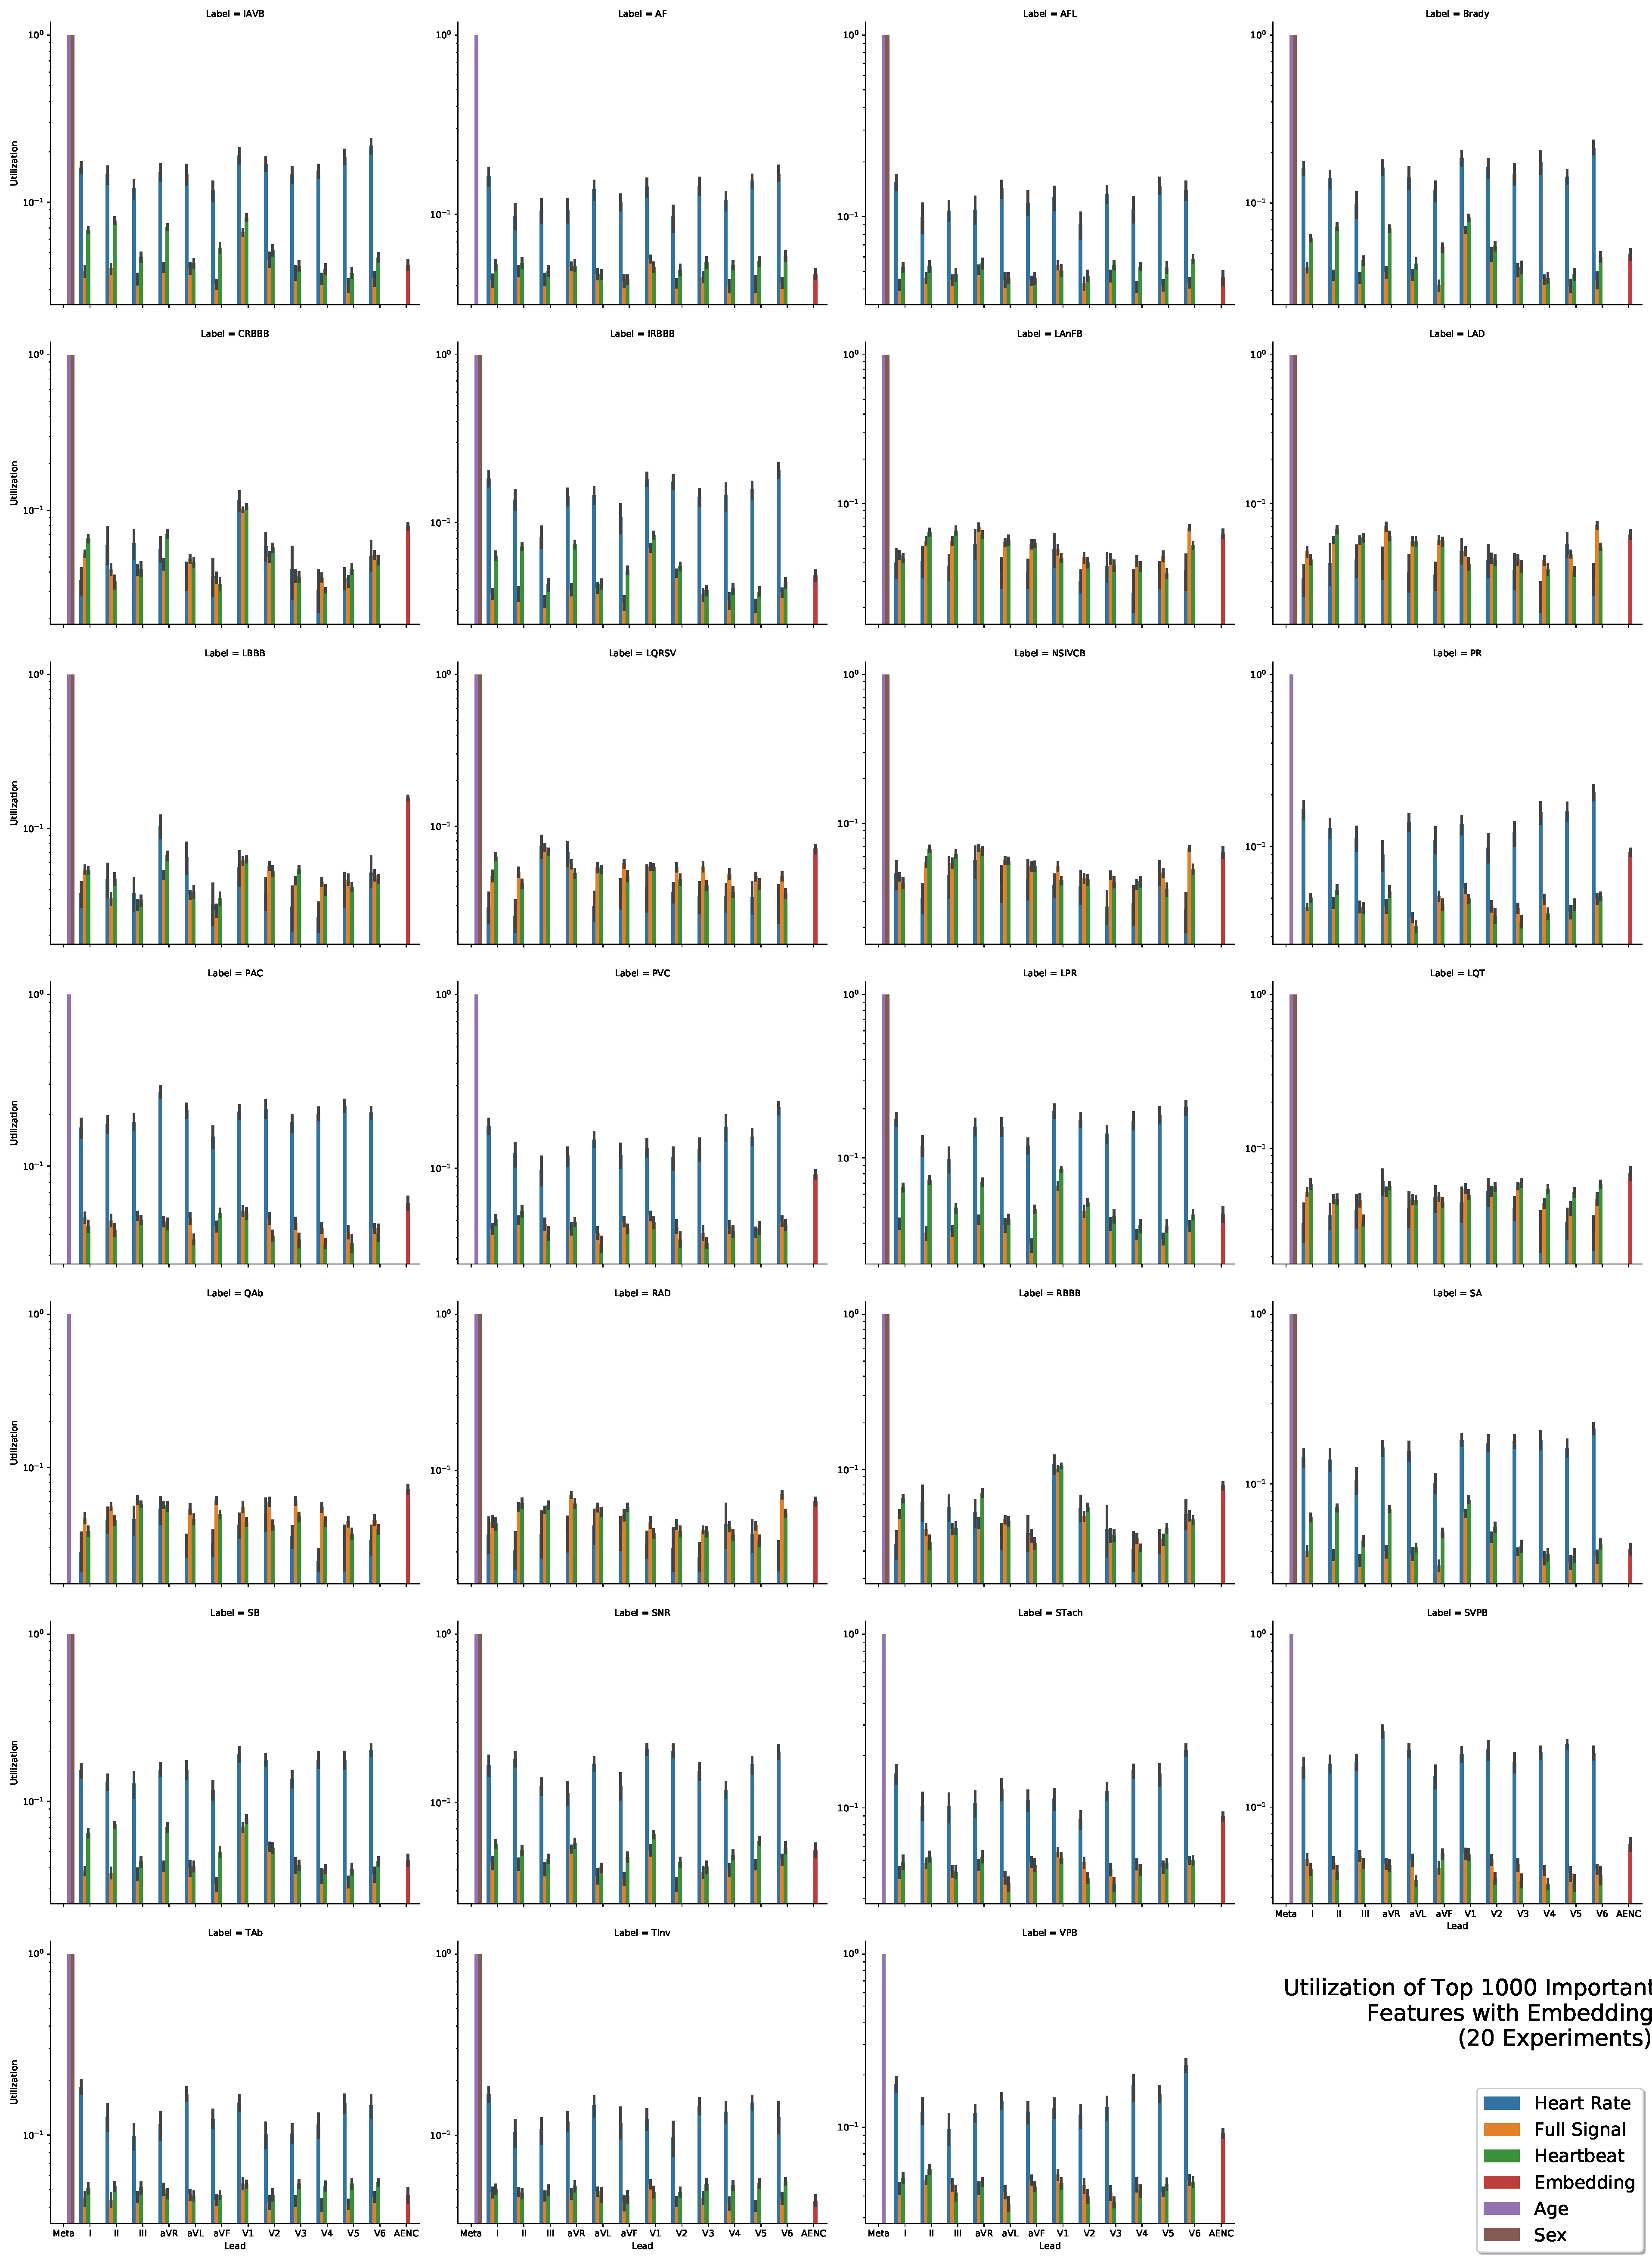
\includegraphics[width=1.1\textwidth]{figure/utilization_top_1000_feature_importances_all_w_embedding.pdf}
    }
    \caption{Feature importances of Configuration~\ref{item:xgb_aenc_model_top_1000_w_embd}: ``Top 1000 Features with Embeddings", utilization over 20 experiments. The 27 diagnosed labels are displayed separately, showcasing feature derived lead (alternatively Meta or Autoencoder), and category.}
    \label{fig:xgb_aenc_top_1000_features_labelwise}
\end{figure}

\begin{figure}[t]
    \centering
    \makebox[\textwidth][c]{
        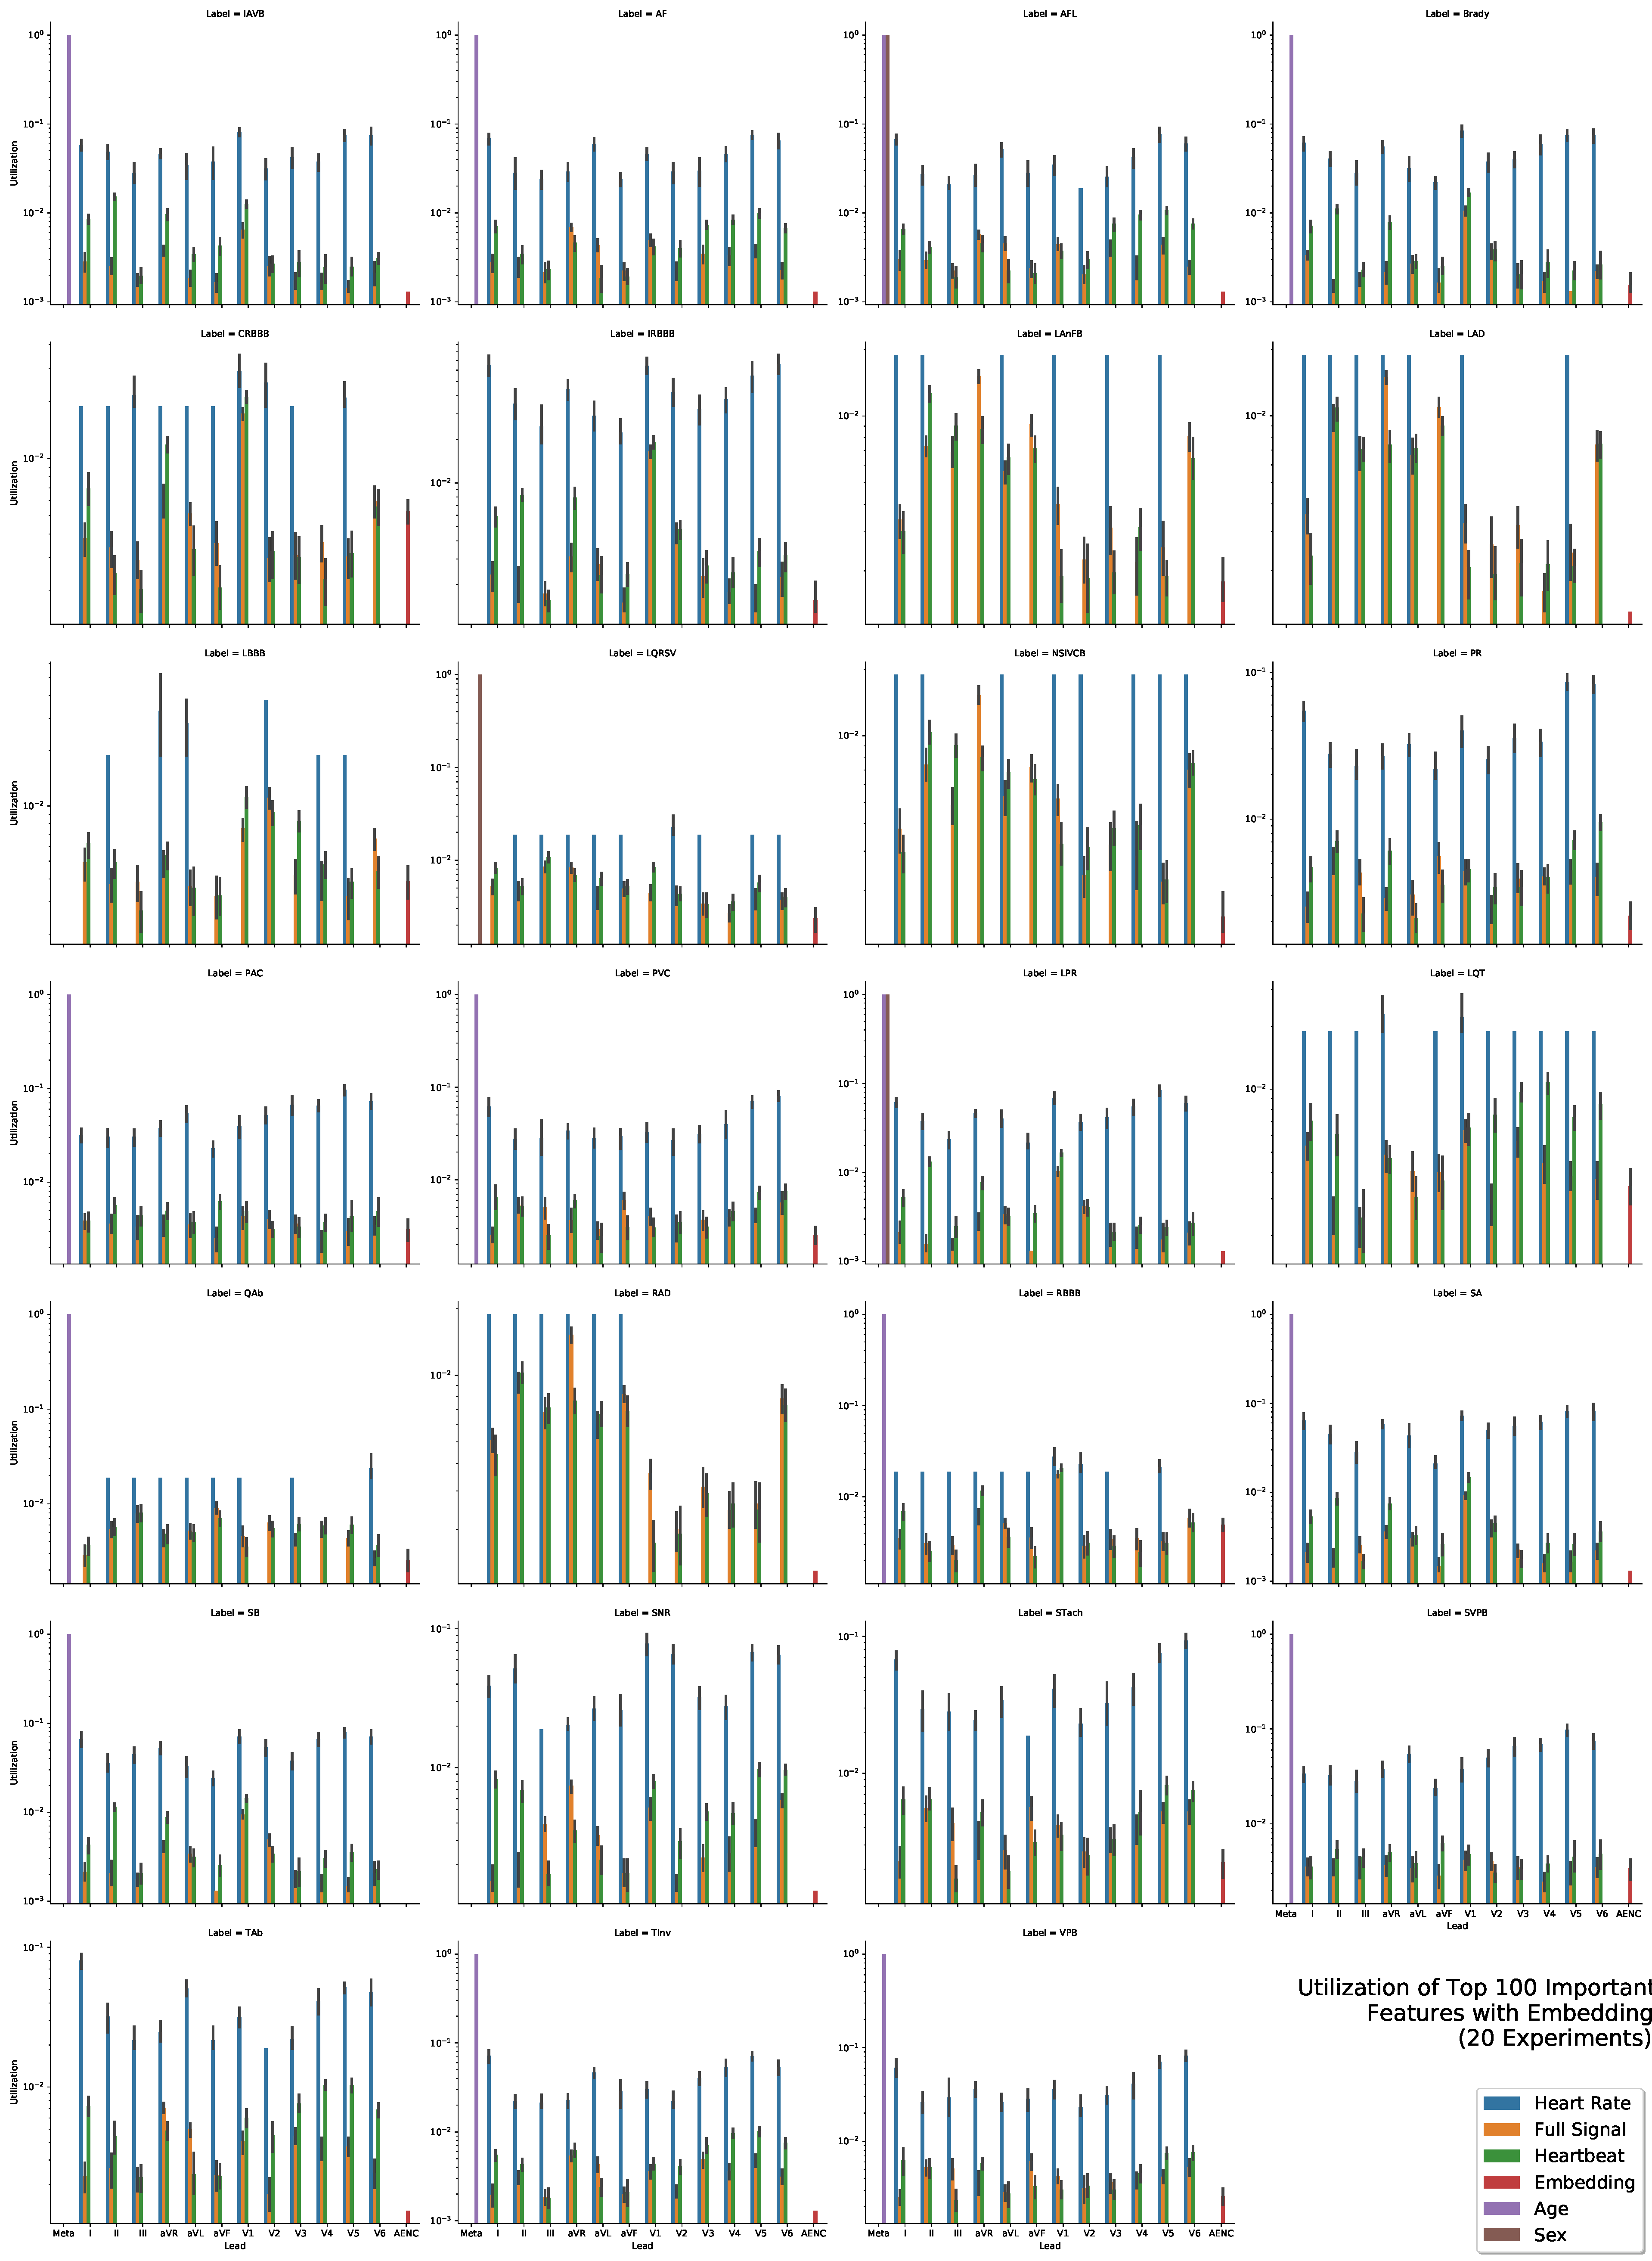
\includegraphics[width=1.1\textwidth]{figure/utilization_top_100_feature_importances_all_w_embedding.pdf}
    }
    \caption{Feature importances of Configuration~\ref{item:xgb_aenc_model_top_100_w_embd}: ``Top 100 Features with Embeddings", utilization over 20 experiments. The 27 labels are displayed separately, showcasing feature derived lead (alternatively Meta or Autoencoder), and category.}
    \label{fig:xgb_aenc_top_100_features_labelwise}
\end{figure}

\end{appendices}
\end{document}
